\documentclass[border=6pt]{standalone}
\usepackage{tikz}
\usetikzlibrary{arrows.meta,positioning,calc,shapes.geometric,fit,backgrounds,patterns,matrix,decorations.pathreplacing}
\begin{document}
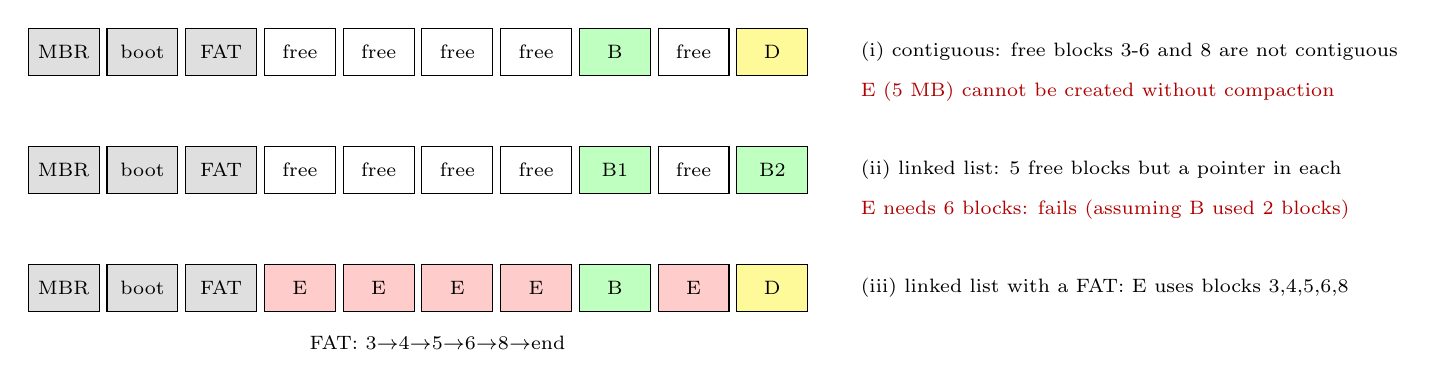
\begin{tikzpicture}[>=Stealth,font=\small]
\tikzstyle{b}=[draw,minimum width=0.9cm,minimum height=0.6cm,font=\scriptsize]
\foreach \r/\y in {0/0,1/-1.5,2/-3.0} { \foreach \i/\n in {0/MBR,1/boot,2/FAT} \node[b,fill=gray!25] at (\i,\y) {\n}; }
\node[font=\scriptsize,anchor=west] at (10,0) {(i) contiguous: free blocks 3-6 and 8 are not contiguous};
\foreach \i/\n/\c in {3/free/white,4/free/white,5/free/white,6/free/white,7/B/green!25,8/free/white,9/D/yellow!40} \node[b,fill=\c] at (\i,0) {\n};
\node[font=\scriptsize,red!70!black,anchor=west] at (10,-0.5) {E (5 MB) cannot be created without compaction};
\node[font=\scriptsize,anchor=west] at (10,-1.5) {(ii) linked list: 5 free blocks but a pointer in each};
\foreach \i/\n/\c in {3/free/white,4/free/white,5/free/white,6/free/white,7/B1/green!25,8/free/white,9/B2/green!25} \node[b,fill=\c] at (\i,-1.5) {\n};
\node[font=\scriptsize,red!70!black,anchor=west] at (10,-2.0) {E needs 6 blocks: fails (assuming B used 2 blocks)};
\node[font=\scriptsize,anchor=west] at (10,-3.0) {(iii) linked list with a FAT: E uses blocks 3,4,5,6,8};
\foreach \i/\n/\c in {3/E/red!20,4/E/red!20,5/E/red!20,6/E/red!20,7/B/green!25,8/E/red!20,9/D/yellow!40} \node[b,fill=\c] at (\i,-3.0) {\n};
\node[font=\scriptsize,anchor=west] at (3,-3.7) {FAT: 3$\to$4$\to$5$\to$6$\to$8$\to$end};
\end{tikzpicture}
\end{document}
